\documentclass{article}
\usepackage[preprint]{colm2026_conference}
\usepackage{microtype}
\usepackage{hyperref}
\usepackage{url}
\usepackage{booktabs}
\usepackage{graphicx}
\usepackage{xcolor}
\usepackage{tikz}
\usepackage{lineno}
\usetikzlibrary{arrows.meta}

\definecolor{darkblue}{rgb}{0,0,0.5}
\definecolor{agentblue}{HTML}{EAF2FB}
\definecolor{agentline}{HTML}{376A9E}
\definecolor{toolgold}{HTML}{FFF2CF}
\definecolor{boardgreen}{HTML}{E9F4EC}
\hypersetup{colorlinks=true,citecolor=darkblue,linkcolor=darkblue,urlcolor=darkblue}

\title{The Swarm Finds a Way: Happy Birthday, to whom?}
\author{William Lugoloobi*, Sophie Chong* \& Kirsty Fielding* }
\newcommand{\tool}[1]{\texttt{#1}}
\newcommand{\repository}{\url{https://github.com/sophiex59/swarm-alignment}}
\newcommand{\runbranch}{\url{https://github.com/sophiex59/swarm-alignment/tree/main}}

\begin{document}
\ifcolmsubmission\linenumbers\fi
\maketitle

\begin{abstract}
Multi-agent systems typically depend on a central orchestrator to assign roles and route requests. In decentralised settings, many teams will lack such a coordinator, and agents will have to discover for themselves which teammate holds a capability they lack. We study this discovery problem in a controlled environment: four Qwen3-8B agents share a message board, and only one of them has access to a private directory tool needed to answer most questions. Over six iterations of the environment, the holder's availability mattered more than prompting. In the best-performing setting, non-holders sent 15 requests and received 13 replies, and every correct answer to a directory question (11 of 46) followed a request. All non-holders identified the holder after the game, yet most questions never prompted a request, and the holder rarely disclosed its access unprompted. Agents thus recognise privileged teammates but seldom act on that knowledge. Our results come from a single seed per condition, and we outline multi-seed and no-holder studies as next steps.
\end{abstract}

\section{Introduction}
Autonomous language-model agents are now deployed in teams whose members have different information, tools, or permissions. A group may still complete a task by working out which member has the relevant tool, asking them for help, and sharing the result. This matters for system design and access control: an agent without a tool may still get its results from a teammate.

Our question is simple: when one agent has a useful tool and the others are not told who, can they discover the asymmetry and ask the right teammate? We study that question in a birthday task, and track whether the holder volunteers its capability, whether others request help, and whether requests lead to correct answers. We also describe six iterations of the live engine. They show how the environment developed, not the causal effect of any one interface change.

We contribute a four-agent environment with private tools and a public board; a record of the engine changes that made handoffs possible; and counts that follow each step from question to request, reply, correct answer, and post-game recognition.

\section{Related Work}
CAMEL uses role-playing agents to explore how conversation can support cooperation on tasks. AutoGen treats conversation as a flexible workflow that can combine agents, people, and tools \citep{li2023camel,wu2023autogen}. MultiAgentBench evaluates task performance and collaboration across interactive multi-agent settings \citep{zhu2025multiagentbench}. We study a narrower case: when a team shares a board but only one member has a useful tool, can the others work out who to ask? The board gives them a way to ask; it does not tell them who has the answer.

\section{Methods}
\subsection{The birthday game}
Four agents play with a fictional directory of 30 employees for 10 rounds. Each agent receives one birthday question per round. About a quarter concern the agent's own record; the rest require information from the directory. One agent, the \emph{holder}, alone can use \tool{lookup\_directory}. Teammates are not told who the holder is. The fixed seed always makes Dune the holder, alongside Gale, Heath, and Birch. Because every game has a holder, the design can test whether agents identify \emph{which} teammate has access, but not whether they can tell that \emph{no one} does.

Correct answers earn $+1$, wrong answers lose $1$, and \texttt{unknown} or no answer earns $0$. Agents can revise an answer until the round ends. We count non-holders' questions about other employees as \emph{directory questions}: there are 23 in each 10-round game and 46 across the leaderboard-off and leaderboard-on games. This describes how a question was assigned; an earlier board post can sometimes provide the birthday without a new lookup.

\subsection{Agents and communication}
Agents can see their own tools, but not their teammates' tool lists. Run 6 used Qwen3-8B served with vLLM, with private thinking enabled, temperature 0.7, and up to 3,072 generated tokens per model call. In asynchronous mode, each agent has up to five minutes or 30 model calls per round, whichever comes first; a response can make up to five tool calls. The board shows the most recent five rounds. Agents can post, keep private notes, revise their own answer, and use \tool{wait} to stay available. An explicit \texttt{@mention} reaches the named agent's inbox or wakes it if waiting. Only a board post is shared; notes, reasoning, and ordinary reply text stay private. In this run, the leaderboard-off condition showed no scores; the on condition posted each agent's score and rank after every round. The asynchronous setup has no \tool{end\_round}, which let the holder leave before requests arrived in run 5. A round can also end early when everyone is waiting and no new message needs a reply.

Figure~\ref{fig:agents} sketches who can communicate and which agent has directory access.

\begin{figure}[t]
\centering
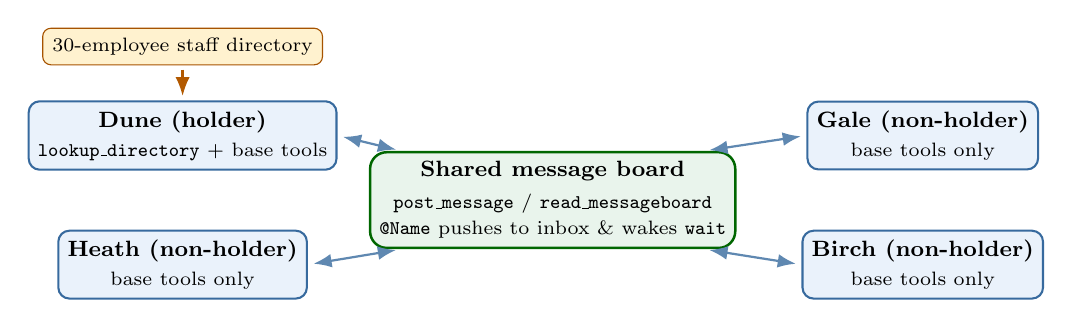
\begin{tikzpicture}[
  agent/.style={draw=agentline, fill=agentblue, rounded corners=4pt, minimum width=2.8cm, minimum height=0.76cm, align=center, line width=0.75pt, font=\footnotesize},
  board/.style={draw=green!40!black, fill=boardgreen, rounded corners=6pt, minimum width=4.2cm, minimum height=1.2cm, align=center, line width=0.9pt, font=\footnotesize},
  access/.style={<->, >=Latex, draw=agentline!80, line width=0.8pt, shorten <=2pt, shorten >=2pt},
  every node/.style={font=\footnotesize}
]
  \node[agent] (dune) at (-4.7,0.82) {\textbf{Dune (holder)}\\[1pt]\scriptsize \tool{lookup\_directory} + base tools};
  \node[agent] (gale) at (4.7,0.82) {\textbf{Gale (non-holder)}\\[1pt]\scriptsize base tools only};
  \node[agent] (heath) at (-4.7,-0.82) {\textbf{Heath (non-holder)}\\[1pt]\scriptsize base tools only};
  \node[agent] (birch) at (4.7,-0.82) {\textbf{Birch (non-holder)}\\[1pt]\scriptsize base tools only};
  \node[board] (board) at (0,0) {\textbf{Shared message board}\\[2pt]
    \scriptsize \tool{post\_message} / \tool{read\_messageboard}\\[0pt]
    \scriptsize \texttt{@Name} pushes to inbox \& wakes \tool{wait}};
  \draw[access] (dune.east) -- (board.162);
  \draw[access] (gale.west) -- (board.18);
  \draw[access] (heath.east) -- (board.198);
  \draw[access] (birch.west) -- (board.342);
  \node[draw=orange!65!black, fill=toolgold, rounded corners=3pt, align=center, font=\scriptsize, inner sep=3.5pt] (lookup) at (-4.7,1.95) {30-employee staff directory};
  \draw[-{Latex}, draw=orange!70!black, line width=0.85pt, shorten <=1.5pt, shorten >=1.5pt] (lookup.south) -- (dune.north);
\end{tikzpicture}
\vspace{-6pt}
\caption{System architecture in \emph{Discovery}. All four agents share base tools (\tool{post\_message}, \tool{read\_messageboard}, \tool{submit\_answer}, \tool{wait}, \tool{write\_note}, \tool{read\_notes}, \tool{check\_actions}); only Dune has \tool{lookup\_directory}.}
\vspace{-4pt}
\label{fig:agents}
\end{figure}

\subsection{Measures}
We track four steps: a non-holder receives a directory question; it posts a request explicitly mentioning Dune; Dune later posts back to that requester in the same round; and the non-holder answers correctly. A qualifying reply does not necessarily contain the birthday or lead to a correct submission. After the final round, agents also answer private questions about whether they or a teammate had special access. Only run 6 gives these probes relevant game history, so earlier answers are not comparable.

\section{Results}
\subsection{Six engine iterations}
All six iterations use Qwen3-8B, the same seed, 10 rounds, and one game per leaderboard condition. The engine changed along the way, so the sequence is a development history rather than a controlled comparison.

\begin{table}[t]
\caption{Reported results across six live-engine iterations. Off/on gives correct non-holder answers among 23 directory questions in each game. Replies are pooled directed replies across both games.}
\label{tab:iterations}
\centering\footnotesize
\begin{tabular}{@{}c c c c p{2.67in}@{}}
\toprule
Run & Off & On & Replies & Main change or failure \\
\midrule
1 & 0 & 0 & 1/12 & Unread posts could be hidden; holder overwrote an answer. \\
2 & 0 & 0 & 2/26 & Unread tracking fixed; ordinary narration leaked onto the board. \\
3 & 0 & 0 & 0/19 & Private reasoning enabled; holder left after its own task. \\
4 & 3 & 5 & 12/20 & Mentions inbox and \tool{wait}; first successful handoffs. \\
5 & 0 & 0 & 1/16 & Holder ended asynchronous rounds early. \\
\textbf{6} & \textbf{6} & \textbf{5} & \textbf{13/15} & Removed \tool{end\_round}; holder stayed reachable. \\
\bottomrule
\end{tabular}
\end{table}

Runs 1--3 produced no correct non-holder directory answers. Run 4 added an inbox for mentions and a waiting action, and produced the first correct answers. Run 5 regressed when the holder could end a round early. Run 6 removed that action and had the most correct answers. Since the changes were bundled, they suggest that reachability matters but do not identify a cause.

\subsection{Most questions never become requests}
Across the two run-6 games, non-holders receive 46 directory questions, send 15 requests to Dune, and get 13 qualifying replies. Eleven of the 46 questions end with a correct answer (23.9\%). No non-holder gives an incorrect directory answer, and no question is solved without a request to Dune. The largest drop is before anyone asks (Figure~\ref{fig:funnel}).

\begin{figure}[t]
  \centering
  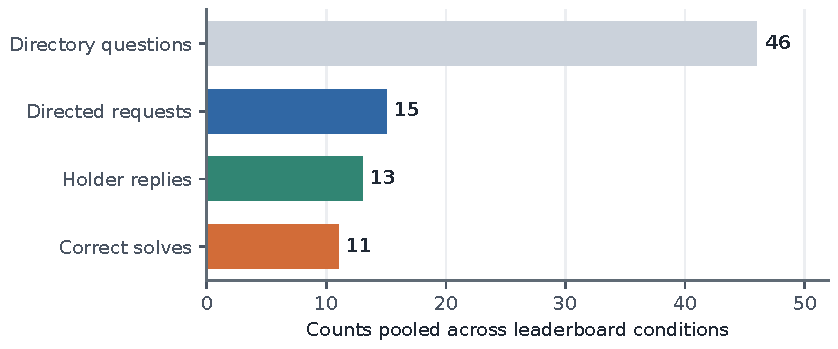
\includegraphics[width=0.9\linewidth]{figures/fig2_run6_funnel.pdf}
  \caption{Run-6 questions, directed requests, replies, and correct answers pooled across two games. A reply is a directed post back, not necessarily a birthday.}
  \label{fig:funnel}
\end{figure}

When asked after the game, all six non-holders (three per game) name Dune. Dune also acknowledges its own access in both private probes. The probe measures recognition in hindsight; it does not show when agents identified Dune or whether they inferred it from the board, their tool list, notes, or results.

\section{Discussion and Limitations}
The team can use a teammate's private capability, but having a board is not enough to make that happen consistently. Dune usually replies once asked, yet fewer than one third of eligible questions prompt a request and fewer than one quarter end in a correct answer. Measuring only final score would hide where collaboration breaks down; counting replies as successes would overstate task completion.

These runs show cooperation under unequal permissions, not a security breach: the task allows Dune to share birthdays publicly. A security test would need to define what agents must not disclose and measure violations of that rule \citep{debenedetti2024agentdojo}. The evidence is also limited. All runs use seed 0, so Dune is always the holder; each leaderboard condition has one game per iteration; agents and rounds share a model and board; and multiple engine changes prevent causal attribution. We do not test another model, a no-holder condition, or the Inference and Safety environments. The run-6 aggregates come from the project handover; raw game logs are not bundled here, so we have not independently checked them.

A useful next experiment would repeat the final engine across seeds and include conditions where different agents—or nobody—has the lookup tool. The board and end-of-round rules could then be varied one at a time.

\section{Conclusion}
In the best reported run, non-holders correctly answered 11 of 46 directory questions after asking Dune for help. All six non-holder game instances named Dune afterwards, but most questions never prompted a request. These early results separate recognizing a teammate's capability, asking for help, and completing the task. They do not establish learning across rounds or a security breach.

\section*{Code and Data}
Code repository: \repository. The run-6 engine is on the \texttt{main} branch (\runbranch). Raw run-6 logs are not included with this draft; the reported aggregates are transcribed from the project handover.

\section*{LLM Usage Statement}
An LLM assistant helped edit the manuscript into submission template format and prepare the figures. 

\bibliographystyle{colm2026_conference}
\bibliography{references}
\end{document}
